\chapter{Поддержка создания предметно-ориентированных решений в системе QReal}
\label{chapterImplementation}

В данной главе описываются технологические средства для разработки предметно-ориентированных 
визуальных языков, реализованные под руководством автора в системе QReal. Описаны 
средства для разработки языков с использованием метаредактора (в соответствии с "`классической"' 
методологией): сам метаредактор, редактор конкретного синтаксиса, редактор ограничений, 
редактор правил рефакторингов, средства генерации редакторов и инструментальной поддержки. 
Также описаны реализованные средства поддержки методологии "`метамоделирования на лету"'.

\section{Возможности ядра системы QReal}
Прежде чем переходить к описанию средств описания визуальных языков, необходимо кратко 
описать возможности системы, в рамках которой будут работать созданные по метамоделям 
редакторы и средства инструментальной поддержки. DSM-платформа QReal построена по 
модульному принципу: имеется абстрактное ядро, реализующее общую для всех языков функциональность 
и инфраструктуру редакторов, в него как подключаемые модули (плагины) загружаются редакторы, 
реализующие специфику конкретных языков, и инструменты, реализующие какую-либо ещё 
специфичную для конкретного DSM-решения функциональность. Ядро не содержит в себе 
никаких знаний про конкретные языки и работает со всеми DSM-решениями одинаковым образом. 
Всю необходимую информацию о языке и действиях, которые можно выполнить над диаграммами, 
созданными с его помощью, ядро получает из плагинов, либо непосредственно из метамодели 
языка, если ядро работает в режиме интерпретации метамодели. Общая архитектура системы 
представлена на рисунке~\ref{qRealArchitecture}.

\begin{figure} [ht]
	\begin{center}
		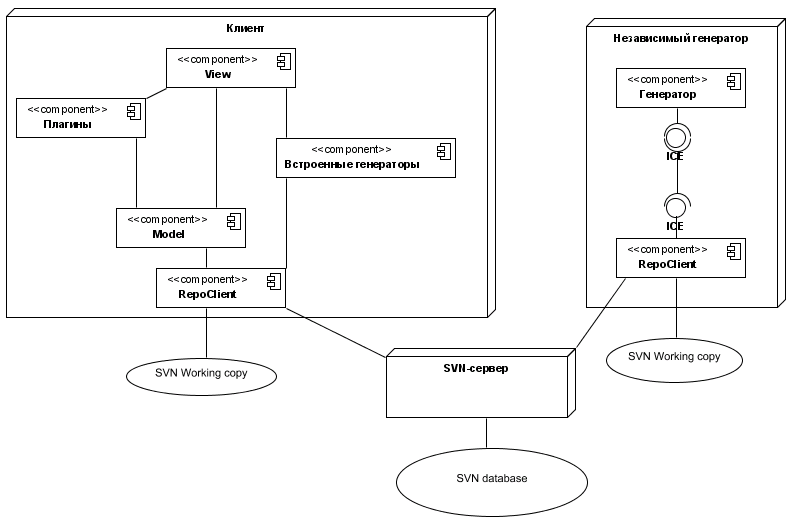
\includegraphics[width=0.7\textwidth]{part4/qRealArchitecture.png}
		\caption{Общая архитектура системы QReal.}
		\label{qRealArchitecture}
	\end{center}
\end{figure}

Плагины-инструменты могут настраивать внешний вид и состав интерфейса QReal под свои 
нужды, базовый интерфейс среды представлен на рисунке~\ref{qRealUi}. Интерфейс содержит 
область для редактирования диаграммы, называемую сценой, редактор свойств, палитру 
элементов, обозреватели логической и графической моделей, "`миникарту"', панель инструментов и меню.

\begin{figure} [ht]
	\begin{center}
		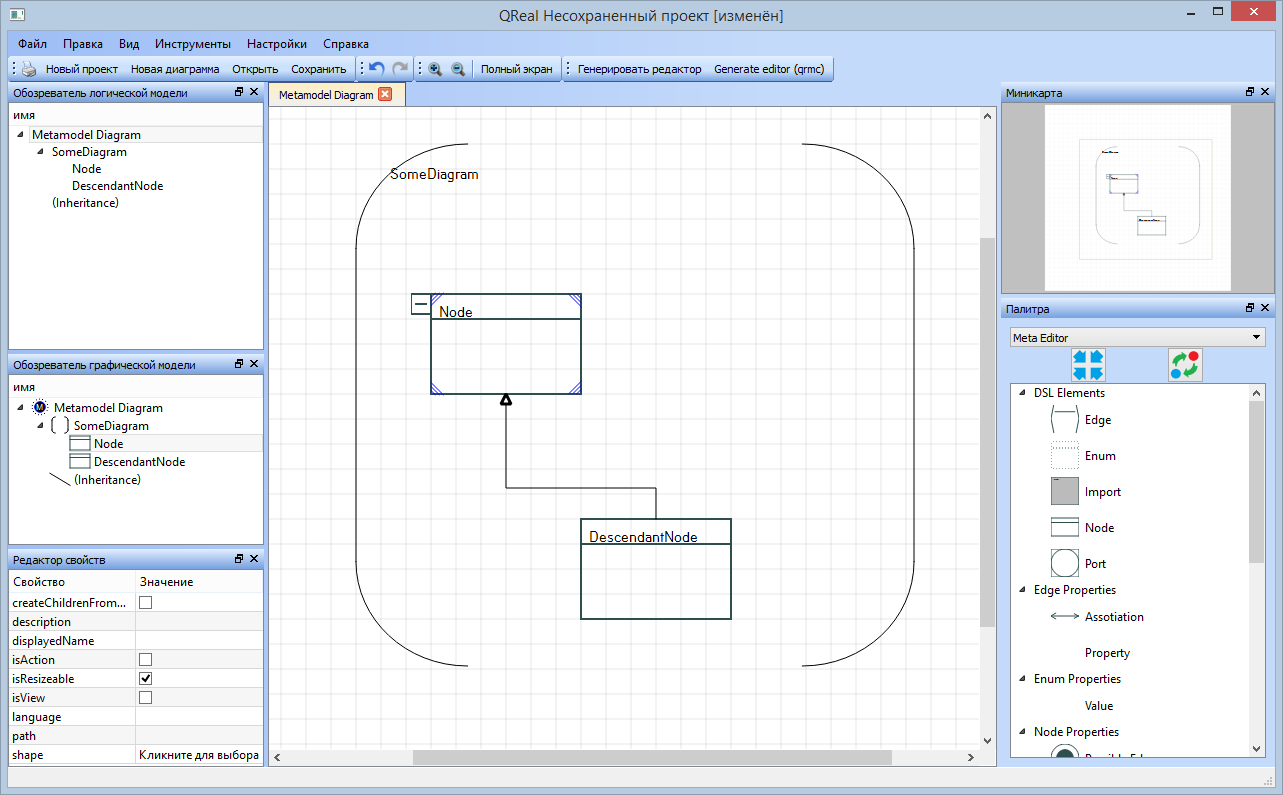
\includegraphics[width=\textwidth]{part4/qRealUi.png}
		\caption{Пользовательский интерфейс системы QReal.}
		\label{qRealUi}
	\end{center}
\end{figure}

Палитра элементов инициализируется описанными в плагине-редакторе элементами. Одновременно 
могут быть подключены несколько плагинов, тогда создаётся  несколько палитр, между 
которыми можно переключаться с помощью выпадающего списка. В палитру попадают только 
те элементы, которые имеют графическое представление, элементы, которые его не имеют, 
считаются абстрактными и используются в качестве базовых для определения других элементов.

Редактор свойств отображает все свойства выделенного в данный момент элемента и даёт 
возможность их редактировать. Свойство характеризуется своим именем (задаваемым в метамодели), 
типом (одним из фиксированного набора элементарных типов, типом-перечислением или 
типом-ссылкой на другой элемент диаграммы) и значением по умолчанию. Для разных типов 
редактор свойств предлагает разные средства редактирования, например, выпадающие списки 
для типов-перечислений, поля ввода для строк, "`галочки"' для булевых свойств.

Панель инструментов содержит элементы, общие для всех редакторов (сохранение/загрузка, 
отмена операции и т.д.), и область, в которую добавляются действия из плагинов-инструментов. 
Действие может вызвать произвольный код из плагина, который может использовать достаточно 
богатый программный интерфейс ядра QReal, предоставляющий доступ к сохранённой в репозитории 
модели, сцене (например, возможность подсветки указанного элемента на сцене), возможность 
подписываться на системные события (например, закрытие вкладки с диаграммой, изменение 
системных настроек).

Любой редактор визуального языка обязан реализовывать определённый интерфейс, чтобы 
быть подключенным к ядру системы. Этот интерфейс определяет информацию, которую настраиваемый 
визуальный редактор, входящий в ядро системы, должен знать о синтаксисе визуального 
языка, чтобы давать возможность создавать диаграммы. С точки зрения ядра системы подключаемый 
визуальный редактор представляет собой набор диаграмм (различных визуальных языков, 
входящих в состав редактора, их может быть несколько), каждая диаграмма содержит в 
себе список элементов. Элемент может быть либо узлом, либо связью. Любой элемент обладает 
списком свойств (свойства с точки зрения абстрактного синтаксиса представляют собой 
тройки "`имя - тип - значение по умолчанию"') и внешним видом. Внешний вид узла задаётся в векторном графическом формате, близком к SVG
% TODO: Ссылка
, но с некоторыми расширениями (возможностью определить порты, к котором могут подключаться связи и областями для вывода значений 
свойств из репозитория). Внешний вид связи определяется стилем линии (сплошная, пунктирная 
и т.д.) и видом конца линии, выбираемым из нескольких предопределённых значений (открытая 
и закрытая стрелки, закрашенный и незакрашенный ромб и т.д.). Для узла также указывается, 
какие связи можно к нему подключить и какие узлы он может содержать внутри себя как 
составные элементы.

Редактор визуального языка можно создать вручную, реализовав описанный выше интерфейс 
на языке C++ и собрав подключаемую библиотеку. Однако такой подход весьма неэффективен, 
поэтому был использован лишь однажды, для нужд тестирования системы. Далее речь пойдёт 
об автоматизации создания визуальных редакторов. Здесь был дан лишь краткий обзор 
возможностей ядра системы, необходимый для дальнейшего изложения, более подробно 
см. диссертацию Брыксина Т.А.
%TODO: Ссылка

\section{Метаредактор}
В системе QReal для быстрого создания редакторов используется визуальный метаязык и 
соответствующий редактор, называемый метаредактором. По визуальной метамодели языка, 
созданной в метаредакторе, генерируется код на C++, реализующий интерфейс подключаемого 
модуля, который требуется ядру системы.

\subsection{Визуальный метаязык}
В основу метаязыка системы QReal заложены принципы, используемые, например, в метаязыке MOF 
%TODO: ссылка
: элементы моделируемого языка (сущности и связи) моделируются сущностями метаязыка 
(Node и Edge), эти сущности могут быть связаны отношениями наследования и "`является контейнером для"'. 
И сущность, и связь могут иметь свойства, значения для которых можно задавать при 
редактировании модели в редакторе свойств QReal. Имеется ряд вспомогательных элементов 
метаязыка, определяющих поведение элементов языка при взаимодействии с ними пользователя, 
например, позволяет ли контейнер располагать внутри себя элементы произвольным образом, 
или сам располагает элементы подряд друг под другом. Подробнее об имеющихся элементах 
см. в таблице ниже.

\begin{center}
	\begin{longtabu} {| X[1 l m] | X[2 c m] | X[3 m] |}
		\caption{Метаязык системы QReal} \\
		\tabucline-
		Название                    & Внешний вид                                                                     & Описание \\
		\tabucline-
		\endfirsthead
		\tabucline-
		Название                    & Внешний вид                                                                     & Описание \\
		\tabucline-
		\endhead
		\noalign{\vspace{3mm}}\caption{Метаязык системы QReal (многостраничная)} \\
		\endfoot
		\everyrow{\tabucline-}
		Metamodel Diagram           & 
\includegraphics[scale=1]{part4/metalanguage/metamodelDiagram.png}              & Корневой элемент метамодели. Может содержать в себе 
		                                                                                                                узлы Meta Editor Diagram (метамодели языков, входящих в 
		                                                                                                                плагин), свойства этого элемента содержат настройки сборки 
		                                                                                                                редактора, такие как относительный путь к исходным файлам 
		                                                                                                                QReal. \\
		Meta Editor Diagram         & 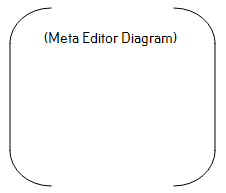
\includegraphics[scale=0.5]{part4/metalanguage/metaEditorDiagram.png}           & Корневой узел метамодели одного визуального языка. Может 
		                                                                                                                содержать в себе узлы Node, Edge, Enum. Для каждого узла 
		                                                                                                                этого типа в метамодели редактора будет сгенерирована своя 
		                                                                                                                вкладка в палитре элементов. \\
		Package Diagram             & 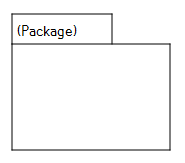
\includegraphics[scale=0.7]{part4/metalanguage/packageDiagram.png}              & Пакет. Предназначен для группировки метамоделей и обеспечения переиспользования 
		                                                                                                                фрагментов метамоделей. Также может быть корневым элементом метамодели. Может  
		                                                                                                                содержать в себе другие пакеты или узлы Metamodel Diagram. На данный момент  
		                                                                                                                функциональность этого узла поддерживается лишь частично и используется в основном для 
		                                                                                                                визуализации зависимостей по включению между метамоделями при импорте их из XML-описаний. \\
		Node                        & 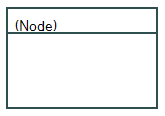
\includegraphics[scale=0.7]{part4/metalanguage/node.png}                        & Представляет узел создаваемого языка. Может содержать в себе узлы Property, Possible Edge, 
		                                                                                                                Properties as Container. Свойства включают в себя имя узла, отображаемое имя узла (с 
		                                                                                                                первым работают генераторы и другие инструменты, отображаемое имя показывается 
		                                                                                                                пользователю), форму узла (форма хранится в виде XML-строки, для её редактирования из 
		                                                                                                                метаредактора открывается редактор формы фигур), некоторые свойства, связанные с 
		                                                                                                                пользовательским интерфейсом (текст всплывающей подсказки для этого узла, может 
		                                                                                                                ли узел менять размер, можно ли создавать вложенные в него узлы с помощью контекстного меню). \\
		Property                    & 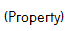
\includegraphics[scale=0.7]{part4/metalanguage/property.png}                    & Свойство. Не имеет какого-либо специального графического оформления, может находиться 
		                                                                                                                только внутри узлов Node и Edge. Для свойства возможно указание имени, отображаемого имени, 
		                                                                                                                типа, значения по умолчанию. Типом свойства может быть один из элементарных типов 
		                                                                                                                (целочисленный, булевый, строковый), тип-перечисление, определённый в этой же
		                                                                                                                метамодели, или ссылочный тип, указывающий на объект типа, определённого в этой же метамодели. \\
		Possible Edge               & 
\includegraphics[scale=0.7]{part4/metalanguage/possibleEdge.png}                & Возможная связь. Указывает, какие элементы мгут быть соединены связью. Задаются имя 
		                                                                                                                узла, из которого может начинаться связь и имя узла, в котором связь может заканчиваться, 
		                                                                                                                также есть возможность указать, направленная связь или нет (то есть можно или нет поменять 
		                                                                                                                начальный и конечый узлы местами). Может находиться внутри узла Node. \\
		Properties as Container     & 
\includegraphics[scale=0.7]{part4/metalanguage/propertiesAsContainer.png}       & Свойства контейнера. Этот элемент отвечает за задание чисто визуальных свойств 
		                                                                                                                взаимодействия узла с вложенными в него узлами, например, должен ли узел  
		                                                                                                                автоматически располагать вложенные узлы друго под другом в столбик, или пользователь 
		                                                                                                                может произвольно располагать вложенные узлы внутри узла-контейнера. Также можно задать 
		                                                                                                                расстояние между вложенными элементами и расстояние от элементов до границы 
		                                                                                                                контейнера, если контейнер сам отвечает за расположение вложенных узлов. Можно указать, 
		                                                                                                                должен ли контейнер автоматически сжиматься или расширяться в соответствии со своим содержимым. \\
		Edge                        & 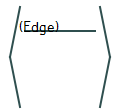
\includegraphics[scale=0.7]{part4/metalanguage/edge.png}                        & Связь. Задаётся имя, отображаемое имя связи, тип линии (сплошная, пунктирная и т.д.), текст, 
		                                                                                                                отображаемый на линии (либо фиксированный, либо свойство связи из репозитория). Кроме  
		                                                                                                                того, связь может иметь свойства, так же как узел. Также можно указать, из какого типа портов 
		                                                                                                                связь может исходить и в какой тип портов связь может входить (см. описание элемента Port). 
		                                                                                                                Если типы портов не указаны, связь может быть подключена к любому порту, если он относится к 
		                                                                                                                допустимому узлу (см. описание элемента Possible Edge). \\
		Association                 & 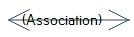
\includegraphics[scale=0.7]{part4/metalanguage/association.png}                 & Элемент для задания свойств начала и конца связи, вкладывается в элемент Edge. Для конца 
		                                                                                                                связи можно указать имя конца и тип стрелки (открытая, закрытая, закрашенная стрелка, 
		                                                                                                                закрашенный и незакрашенный ромб, без стрелки). \\
		Enum                        & 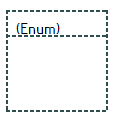
\includegraphics[scale=0.7]{part4/metalanguage/enum.png}                        & Тип-перечисление. Позволяет указать фиксированный набор значений, который можно 
		                                                                                                                использовать как тип какого-либо свойства. Состоит из набора элементов Value. \\
		Value                       & 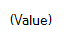
\includegraphics[scale=0.7]{part4/metalanguage/value.png}                       & Одно значение типа-перечисления, вкладывается в элемент Enum. Содержит 
		                                                                                                                только имя значения. \\
		Port                        & 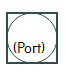
\includegraphics[scale=0.7]{part4/metalanguage/port.png}                        & Объявление типа порта, к которому могут быть подключены определённые связи. При 
		                                                                                                                редактировании формы узла имеется возможность для каждого порта, рисуемого на  
		                                                                                                                изображении узла, указать его тип, а для связи указать тип порта, к которому связь может быть 
		                                                                                                                подключена. \\
		Import                      & 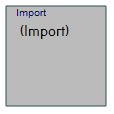
\includegraphics[scale=0.7]{part4/metalanguage/import.png}                      & Импорт элемента. Позволяет использовать элементы одной метамодели в другой 
		                                                                                                                метамодели. Имеется возможность переопределить имя элемента и его  
		                                                                                                                отображаемое имя. \\
		Container                   & 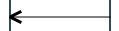
\includegraphics[scale=0.7]{part4/metalanguage/container.png}                   & Связь, задающая допустимую вложенность между элементами. Направлена от элемента, 
		                                                                                                                который может вкладываться в другой, к тому элементу, в который он может вкладываться. По  
		                                                                                                                умолчанию элементы не вкладываются друг в друга. Связь учитывает отношение 
		                                                                                                                наследования, то есть любой потомок вкладываемого элемента может быть вложен в 
		                                                                                                                любой потомок элемента, в который исходный элемент вкладывается. Этим отношением могут 
		                                                                                                                быть связаны только узлы. \\
		Explodes To                 & 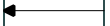
\includegraphics[scale=0.7]{part4/metalanguage/explodesTo.png}                  & Эксплозия, или отноошение раскрытия. Связывает элемент и тот элемент, в который 
		                                                                                                                первый элемент может раскрываться (например, узел, обозначающий подпрограмму, и диаграмму  
		                                                                                                                подпрограммы, в которую он раскрывается). Связь содержит ряд вспомогательных свойств, 
		                                                                                                                например, необходимо ли немедленно создать тот узел, на который ссылается исходный, или 
		                                                                                                                сделать ли связь переиспользуемой (в этом случае узел, соединённый этой связью, 
		                                                                                                                добавляется на пользовательскую палитру и может быть добавлен в других местах 
		                                                                                                                диаграммы или на другие диаграммы, с сохранением связи-раскрытия). Связь также  
		                                                                                                                учитывает отношение наследования. \\
		Inheritance                 & 
\includegraphics[scale=0.7]{part4/metalanguage/inheritance.png}                 & Наследование. Обозначает, что один элемент является подвидом другого элемента и может 
		                                                                                                                быть использован везде вместо своего предка. Наследование означает, что узел-потомок имеет  
		                                                                                                                все свойства узла-предка, а также наследует все отношения вложенности и раскрытия, 
		                                                                                                                которыми был связан предок. Наследование может быть множественным.
		\label{tab:metalanguage}
	\end{longtabu}

\end{center}

\subsection{Особенности языка}
Метаязык QReal имеет следующие особенности, важные для создания CASE-инструментов 
промышленного уровня.

\begin{enumerate}
	\item Принцип "`Если функциональность не требуется, о ней можно не знать"'. Метаредактор 
		определяет ряд разумных умолчаний, так что для создания простого языка достаточно 
		владеть всего несколькими элементами метаязыка. Остальные элементы можно добавлять 
		в метамодель по мере необходимости.
	\item Возможность определения нескольких языков в рамках одной метамодели. Это даёт 
		возможность реализовать подход, при котором проектируемая система рассматривается 
		с нескольких разных точек зрения, которые, тем не менее, взаимосвязаны и подчиняются 
		единым правилам.
	\item Возможность переиспользования фрагментов метамоделей. Это даёт возможность 
		создавать семейства языков, базирующиеся на общей метамодели, а также иметь метамодель-библиотеку 
		для хранения и переиспользования основных конструкций. Особенно полезно это при 
		создании диалектов существующих языков, таких как UML.
	\item Возможность задания отношения вложенности между элементами. Эта возможность 
		является скорее синтаксическим сахаром, поскольку отношение вложенности легко 
		задаётся через связи (два элемента модели, соединённые отношением "`вложен"', 
		семантически эквивалентны одному элементу, вложенному в другой). Тем не менее, 
		это отношение весьма полезно, поскольку работа с элементами-контейнерами и вложенностью 
		требует специальной (и довольно серьёзной) поддержки со стороны редактора.
	\item Типизированные порты дают возможность различать места на фигуре, к которым 
		могут быть подключены связи, и по-разному обрабатывать связи в зависимости от 
		того, к какому конкретно порту они подключены. Потенциально таким портам можно 
		указывать количество подключаемых связей, задавая тем самым языки наподобие электрических 
		схем, но эта возможность в QReal пока не реализована.
	\item Отношение раскрытия (или эксплозия) появилось в метаязыке как обобщение понятия 
		"`провязка"', то есть неграфической связи между элементами. Отношение "`провязка"' 
		позволяло определить произвольную связь между элементами, в том числе и на разных 
		диаграммах, которая могла использоваться, например, для связывания случая использования 
		и диаграммы классов, его реализующей, или класса и реализующей его машины состояний. 
		Кроме того, провязкой же могли связываться элементы, просто "`знающие"' друг о друге, 
		например, узел ветвления и узел объединения ветвей из диаграммы активностей UML. 
		Семантика провязки определялась для каждого конкретного визуального языка. Раскрытие, 
		в отличие от провязки, позволяет явно задать поведение редактора при работе со 
		связанными этим отношением элементами. Также это отношение напрямую связано с 
		пользовательской палитрой --- палитрой, похожей на основную палитру языка, на 
		которую выносятся все созданные пользователем подпрограммы, которые можно использовать 
		как обычные узлы языка. Естественно, это имеет смысл только для языков, в которых 
		определено понятие "`подпрограмма"', поэтому такое поведение задаётся в метаредакторе 
		как свойство отношения раскрытия. Именно с помощью этого отношения реализованы 
		подпрограммы в языке QReal:Robots.
\end{enumerate}

\subsection{Генерация редакторов}
Созданную в метаредакторе метамодель можно использовать для того, чтобы получить редактор, 
несколькими способами: сгенерировать исходный код редактора непосредственно по метамодели, 
сгенерировать сначала XML-описание, а затем по XML-описанию исходный код редактора, 
либо открыть метамодель в интерпретаторе метамоделей и обойтись вовсе без генерации. 
Схематически разные способы представлены на рисунке~\ref{image:editorGeneration}.

\begin{figure} [ht]
	\begin{center}
		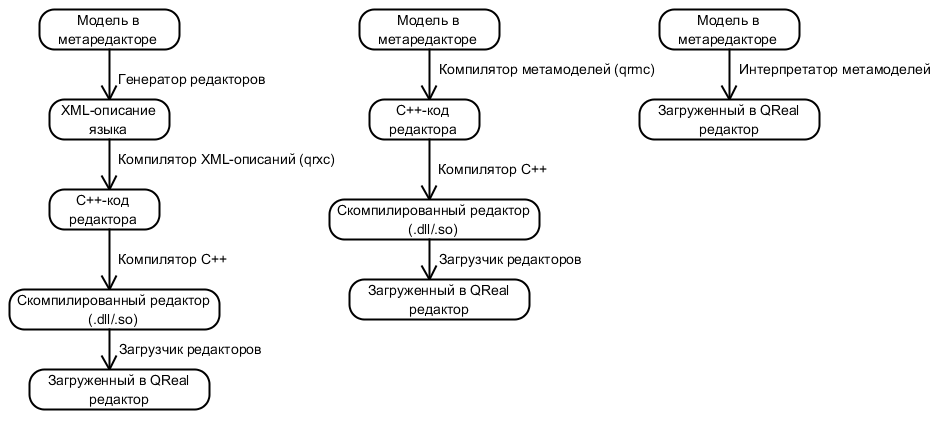
\includegraphics[width=\textwidth]{part4/editorGeneration.png}
		\caption{Получение редактора по метамодели.}
		\label{image:editorGeneration}
	\end{center}
\end{figure}

Способ, использующий XML-описание метамодели, был реализован в QReal первым. Связано 
это с тем, что изначально все описания метамоделей задавались в XML-виде, метаредактор 
появился позднее. Поскольку уже существовала утилита, генерирующая исходный код редактора 
по XML-описанию, сделать генерацию из визуальной метамодели в XML и поддержать в среде 
автоматический запуск утилиты, генерирующей код на C++, а затем самого компилятора, 
оказалось проще. Однако такой подход концептуально сложен: для того, чтобы добавить 
новую функциональность в метаязык, требуется поддержать её в самом визуальном метаязыке, 
в генераторе XML-описания, в утилите, которая генерирует код на C++, и в ядре системы. 
Поэтому было принято решение генерировать код на C++ по метамодели напрямую, и была 
разработана вторая утилита,  принимающая на вход файл с сохранённой метамоделью. Тем 
не менее, система сборки QReal до сих пор использует подход с промежуточным XML-представлением, 
и большинство визуальных языков заданы именно в этом виде. Связано это с тем, что в 
QReal до сих пор не реализован механизм миграции моделей при изменении метамодели 
языка, так что при практически любом изменении в метаязыке уже созданные в нём метамодели 
окажется невозможно открыть в QReal. XML-представление, поскольку легко редактируется 
вручную, гораздо устойчивее к изменениям, так что нет риска оказаться в ситуации, когда 
редакторы невозможно собрать автоматически без ручной правки файлов с сохранениями. 

Структура XML-файла практически полностью соответствует структуре метамодели языка 
(точнее, с исторической точки зрения, наоборот, визуальный метаязык появился как визуализация 
существующего XML-языка). Синтаксис языка был впервые предложен в дипломной работе А.А. Симоновой
%TODO: Ссылка
, однако претерпел с тех пор ряд значительных изменений. Новые возможности ядра QReal 
реализуются сначала в XML-языке, а уже затем переносятся в метаязык, и на данный момент 
XML-язык обладает возможностями, которые в метаязыке пока отсутствуют. Пример такой 
возможности --- задание групп в палитре. Эта возможность позволяют собрать близкие 
по смыслу элементы языка и сворачивать или разворачивать в палитре группы элементов. 
Также есть возможность задать одновременное создание сразу нескольких элементов, например, 
чтобы при создании диаграммы поведения робота на неё сразу же добавлялся блок "`начало"', 
обязательный для всех диаграмм.

Интерпретатор метамоделей позволяет избежать необходимости генерации кода на C++ и 
компиляции редактора. Метамодель языка, подготовленная в метаредакторе, загружается 
в интерпретатор, и он с её помощью эмулирует поведение сгенерированного плагина-редактора. 
При таком подходе скорость работы системы несколько меньше, чем в случае скомпилированного 
редактора, зато отсутствие необходимости пересобирать редактор после каждого изменения 
языка значительно снижает время цикла "`разработка-тестирование"' для вносимых в язык 
изменений. Кроме того, интерпретатор делает возможным внесение в метамодель изменений 
прямо в процессе работы с редактором языка, поэтому применение такого подхода необходимо 
для реализации инструментальной поддержки режима "`метамоделирования на лету"'. Подробно 
реализация интерпретатора метамоделей описана в курсовой работе Птахиной Алины Ивановны
%TODO: Ссылка
. На данный момент в QReal применяется и генеративный, и интерпретативный подходы к 
созданию редакторов, интерпретатор используется для быстрого прототипирования языка, 
генераторы --- для финализации языка и создания инсталляционных пакетов, поставляемых 
пользователям. Для того, чтобы гарантировать, что результирующие редакторы ведут себя 
одинаково для одной метамодели языка вне зависимости от способа получения редактора, 
была разработана и включена в процесс сборки тестирующая система, создающая тестовые 
редакторы для нескольких разных метамоделей всеми тремя способами и проверяющая, что 
все функции интерфейса редактора во всех трёх случаях возвращают одинаковый результат.

\section{Редактор формы фигур}
Редактор формы фигур предназначен для задания конкретного синтаксиса языка и представляет 
собой простой векторный редактор, запускаемый из метаредактора при редактировании свойства 
"`Форма"' узла. Использовать существующие графические редакторы оказалось невозможным 
в связи с тем, что требуется задавать не только внешний вид элемента, но и поведение 
элемента при взаимодействии с ним пользователя --- куда можно подключать связи, как 
должна изменяться форма элемента при его растягивании или сжатии, где выводить значения 
свойств из репозитория.

Пользовательский интерфейс редактора формы фигур представлен на рисунке~\ref{image:shapeEditor}.

\begin{figure} [ht]
	\begin{center}
		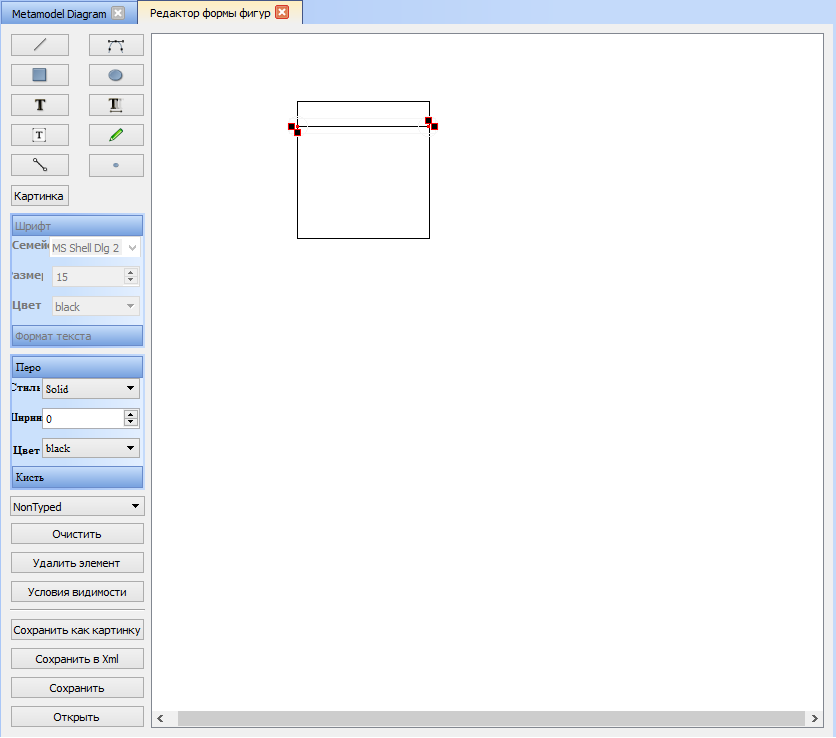
\includegraphics[width=\textwidth]{part4/shapeEditor.png}
		\caption{Редактор формы фигур.}
		\label{image:shapeEditor}
	\end{center}
\end{figure}

Редактор позволяет использовать изображения, заранее подготовленные в обычных графических 
редакторах, в качестве элементов создаваемой формы фигуры, например, так реализованы 
фигуры блоков в QReal:Robots. 

Изображения могут быть дополнены точечными и линейными портами. Порт --- место на 
фигуре, к которому можно подключить связь, точечный порт отличается от линейного тем, 
что к линейному порту связь может подсоединяться в любом месте линии. Порт может иметь 
тип, один из заранее определённых в метамодели, связи может быть указано, к портам 
какого типа её разрешено подключать. Для того, чтобы задать тип, надо выделить порт 
и выбрать его тип из выпадающего списка. Значения в этом списке берутся из метамодели.

Имеется возможность задать отображение статического текста, динамического текста и 
текста как картинки. Динамический текст --- поле на фигуре, текст для которого берётся 
из свойства фигуры в репозитории. В редакторе формы фигур указывается имя свойства, 
откуда надо брать значение. В процессе рисования диаграммы на созданном языке подставляется 
реальное текущее значение свойства, кроме того, значение свойства можно редактировать 
прямо на сцене. Статический текст --- это нередактируемая надпись на элементе, выполненная 
в том же стиле, что и динамический текст. В редакторе формы фигур в этом случае указывается 
сам текст, который должен отображаться. Текст как картинка --- это статический текст, 
которому можно указать произвольный шрифт, стиль начертания, цвет и размер, но при 
этом его нельзя редактировать, выделять или перемещать, он ведёт себя просто как элемент 
изображения.

Для каждого элемента изображения можно определить условие, при котором он будет отображаться. 
Условие задаётся в виде логического выражения, в котором можно использовать значения 
свойств элемента. 

Результат создания формы фигуры может быть сохранён в виде XML-строки как свойство 
элемента Node в метамодели, либо как отдельный XML-файл, который можно переиспользовать 
при создании других фигур.

\section{Редактор ограничений}
Ограничения необходимы для того, чтобы, во-первых, минимизировать вероятность ошибок 
при разработке системы, во-вторых, чтобы иметь возможность обнаружить ошибку как можно 
раньше. Наличие средств задания ограничений позволяет существенно повысить удобство 
пользования визуальной технологией и повысить качество программ, создаваемых с её помощью, 
поэтому средства задания ограничений очень распространены в существующих DSM-платформах. 

Ограничения бывают двух видов --- ограничения на состояние разработанной системы во 
время её работы, и ограничения на модель системы в процессе её разработки. Первый 
вид ограничений схож с операторами assert в текстовых языках программирования, второй --- 
с синтаксическими проверками кода, выполняемыми компилятором или средой разработки. 
В случае DSM-платформы первый вид ограничений может быть реализован только для частных 
случаев, в рамках разрабатываемых с помощью DSM-платформы визуальных технологий. Второй 
же вид ограничений может описываться на уровне метамодели визуального языка, в этом 
случае ограничения могут автоматически проверяться редактором диаграмм. Далее речь 
пойдёт исключительно про второй вид ограничений.

Задание ограничений на создаваемую модель в некотором виде происходит в самой метамодели, 
правила синтаксиса языка не позволят создать некорректную диаграмму, если редактор строго 
им следует (что в случае DSM-платформ практически всегда так, потому что редактор 
определяется метамоделью). Насколько сложные ограничения можно задать в метамодели 
языка, зависит от используемого метаязыка, например, в метаязык можно включить понятие 
типа для свойств, тогда редактор не позволит при создании диаграмм задавать свойствам 
значения, не соответствующие их типу. Можно включить в метамодель проверку на соответствие 
значений свойств регулярным выражениям или логическим условиям, можно продолжить обобщать 
такой подход: например, метамодель UML использует для задания ограничений полноценный 
текстовый язык OCL, позволяющий писать сколь угодно сложные запросы к репозиторию с 
моделью и накладывать сколь угодно сложные ограничения на её состояние.

В системе QReal в соответствии с принципом "`не надо знать то, чем не пользуешься"' 
сложные ограничения задаются отдельно от метамодели, с помощью модели ограничений. 
Метамодель может быть создана без ограничений, они могут быть добавлены в язык потом,
по мере осознания разработчиками языка их необходимости, и отдельно, без внесения 
изменений в метамодель. Кроме того, в соответствии с идеологией предметно-ориентированного 
визуального моделирования ограничения задаются с помощью специально созданного для 
этого предметно-ориентированного визуального языка. Данный язык, а также средства 
проверки ограничений, записанных с его помощью, были реализованы в рамках курсовой 
работы Дерипаска Анны Олеговны 
%TODO: Ссылка
под руководством автора данной работы, и подробно описаны в отчёте о курсовой работе и в статье
%TODO: Ссылка, Дерипаска А.О. Языки задания ограничений. // Компьютерные инструменты в образовании, СПб., 2013, № 1, С. 13-26
, ниже приводится лишь краткое описание данных средств.

Модель ограничений создаётся после создания метамодели языка (или совместно с ней), 
также имеется возможность задавать ограничения, проверяемые для всех метамоделей (например, 
что связи должны быть обязательно подсоединены к узлам). Модель ограничений состоит 
из набора ограничений на узлы и связи. Для каждого узла или связи возможно указать 
ограничения на значение его свойств, для узла можно указать ограничения на входящие 
и исходящие связи, на содержащиеся в узле элементы или наоборот, на содержащий узел 
элемент, для связи --- на узлы, с которых начинается или которыми заканчивается связь. 
Для каждого ограничения можно указать его важность --- предупреждение или критическая 
ошибка. В случае нарушения ограничения-предупреждения элемент-нарушитель подсвечивается 
на диаграмме, в случае нарушения критического ограничения в дополнение к подсветке в 
окне ошибок появляется текстовое сообщение. 

Пример простого ограничения, применимого ко всем типам связей всех метамоделей, приведён 
на рисунке~\ref{image:constraintExample}. Ограничение требует, чтобы у любой связи существовал и начальный, и конечный 
узел (зелёный квадрат означает узел, из которого исходит связь, красный --- узел, в 
который связь входит, true означает, что они должны существовать). Ограничение имеет 
важность "`предупреждение"'.

\begin{figure} [ht]
	\begin{center}
		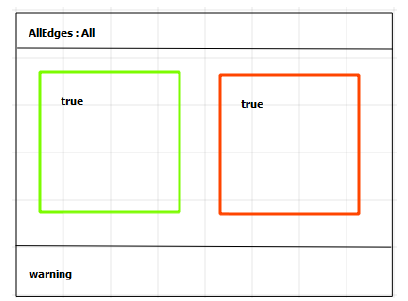
\includegraphics[width=0.5\textwidth]{part4/constraintExample.png}
		\caption{Ограничение, проверяющее наличие начального и конечного узла у связи.}
		\label{image:constraintExample}
	\end{center}
\end{figure}

Пример диаграммы с нарушением этого ограничения приведён на рисунке~\ref{image:constraintViolationExample}. 
Связь, не имеющая конечного узла, выделена средством проверки ограничений красным.

\begin{figure} [ht]
	\begin{center}
		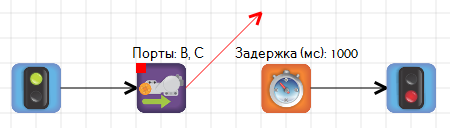
\includegraphics[width=0.7\textwidth]{part4/constraintViolationExample.png}
		\caption{Пример отображения нарушения ограничения.}
		\label{image:constraintViolationExample}
	\end{center}
\end{figure}

Механизм проверки ограничений реализован следующим образом. По модели ограничений 
генерируется код подключаемого модуля проверки ограничений на C++, который компилируется 
в динамическую библиотеку. При запуске QReal все модули проверки ограничений загружаются 
в подсистему проверки ограничений ядра QReal. При выполнении пользователем определённых 
действий (таких как изменение имени элемента, изменение значения свойства элемента, 
создании или удалении элемента, подключение или отключение связи) вызывается обработчик 
в подсистеме проверки ограничений. Обработчик быстро проверяет наличие ограничения 
на тип изменённого элемента в списке подключённых модулей проверки, а также для всех 
связей и содержащих элемент элементов, и наоборот, элементов, содержащихся в данном. 
В случае, если в подключённых модулях хоть одно такое ограничение есть, для каждого 
ограничения вызывается его проверка, результаты собираются в список и, если есть невыполненные 
ограничения, информация об этом предоставляется пользователю в виде подсветки элементов 
на диаграмме и, возможно, в текстовом виде в окне ошибок. Таким образом, несмотря на то, 
что проверка ограничений вызывается при практически любом редактировании модели, за 
счёт фильтрации ограничений по типу проверяемого объекта это не приводит к существенной 
потере производительности.

\section{Редактор правил рефакторинга}
Возможность автоматически применять рефакторинги для диаграмм довольно редка среди CASE-систем и DSM-платформ
%TODO: Уточнить, где такое бывает
, но стала вполне обычной для текстовых сред программирования, поэтому ожидается и от создаваемых визуальных сред, чтобы успешно конкурировать с текстовыми. 
Рефакторинг определяется как изменение внутренней структуры программы без изменения 
её видимого поведения с целью сделать её проще для понимания и упростить её сопровождение
%TODO: тут ссылка на книжку Фаулера про рефакторинг
. В случае с визуальными моделями рефакторинг может рассматриваться как изменение логической 
модели системы или как изменение внешнего вида диаграммы, не затрагивающее логическую 
модель (например, перерасположение элементов). Второй вид рефакторинга исследован 
достаточно хорошо (см. Dot, KIELER и т.д.)
% TODO: Ссылки
, и система QReal использует стороннюю компоненту GraphViz 
% TODO: Ссылка
для автоматической раскладки элементов на диаграммах. Первый вид рефакторингов изучен 
гораздо меньше.

В общем случае схема рефакторинга визуальной модели такова.
%TODO: ссылка на Tom Mens, Gabriele Taentzer, Dirk Müller, Challenges in Model Refactoring. // Proc. 1st Workshop on Refactoring Tools University of Berlin (2007), pp.75-81
 Система состоит из нескольких визуальных моделей, характеризующих систему с разных точек зрения, по моделям автоматически 
генерируется часть кода, другая часть кода, возможно, пишется вручную. При рефакторинге 
необходимо, во-первых, внести необходимые изменения в редактируемую модель, во-вторых, 
синхронизировать изменения с другими моделями, в-третьих, выполнить перегенерацию кода 
по моделям, затронутым изменениями, в-четвёртых, согласовать рукописный код. Рефакторинг 
вручную может оказаться весьма трудоёмким процессом, поэтому естественно желание его 
автоматизировать. Но для каждого визуального языка набор рефакторингов может быть свой, 
зависящий от семантики конкретного языка. Поэтому требуется задавать правила рефакторингов 
на уровне метамодели. В QReal для задания рефакторингов принят тот же подход, что и 
для задания ограничений --- правила рефакторингов, если они требуются, определяются 
в отдельной модели после определения метамодели языка, для этого используется специализированный 
визуальный язык. Этот визуальный язык и средства, позволяющие применять заданные с его 
помощью рефакторинги, был реализован в рамках курсовой работы Кузенковой Анастасии Сергеевны 
под руководством автора данной работы. Ниже приводится краткое описание реализации 
системы рефакторингов в QReal, подробнее см. в отчёте по курсовой работе
% TODO: Ссылка
, а также в статьях
% TODO: Ссылка
% Кузенкова А.С., Литвинов Ю.В. Поддержка механизма рефакторингов в DSM-платформе QReal // Материалы межвузовского конкурса-конференции студентов, аспирантов и молодых ученых Северо-Запада "Технологии Microsoft в теории и практике программирования". СПб.: Изд-во СПбГПУ, 2013. С. 71-72
% Кузенкова А.С., Поддержка механизма рефакторингов в metaCASE-системе QReal // Список-2012: Материалы всероссийской научной конференции по проблемам информатики. 25-27 апр. 2012г., Санкт-Петербург. — СПб.: Изд-во ВВМ, 2012. С. 24-33
. Общая схема разработки и применения правил рефакторинга представлена на рисунке~\ref{image:refactoring}.

\begin{figure} [ht]
	\begin{center}
		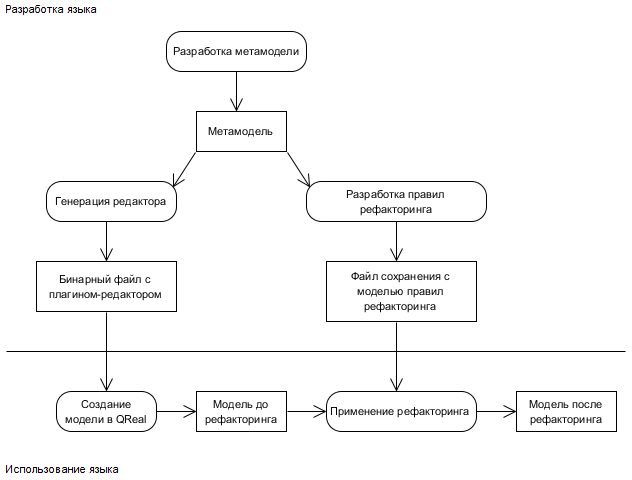
\includegraphics[width=\textwidth]{part4/refactoring.png}
		\caption{Схема разработки и применения правил рефакторинга.}
		\label{image:refactoring}
	\end{center}
\end{figure}

Язык описания правил рефакторинга имеет интересную особенность --- его элементами 
являются элементы языка, для которого определяется правило рефакторинга. Эти элементы 
автоматически подгружаются из метамодели разрабатываемого языка редактором правил 
рефакторинга и используются для определения шаблонов, которые будет сопоставлять в 
диаграмме средство выполнения рефакторинга при его применении. Сами правила задаются 
в виде графовых грамматик: правило делится на часть BEFORE, в которой задаётся шаблон, 
который ищется в диаграмме, и на часть AFTER, на которую замещается сопоставленный 
шаблон. При этом в правиле можно использовать специальные элементы, такие как "`Выделенный 
фрагмент диаграммы"', каждому элементу можно указать его идентификатор. Элементы, 
имеющие одинаковый идентификатор в левой и правой части правила, считаются одним элементом 
и будут сохранены (возможно, с изменениями) при рефакторинге. Элементы, идентификатор 
которых не встречается в части BEFORE, будут созданы, элементы, идентификатор которых 
не встречается в части AFTER --- удалены. Можно модифицировать существующее значение 
свойства элемента, для доступа к нему используется ключевое слово EXISTS. Пример правила 
рефакторинга для метаязыка, который к имени каждого узла приписывает префикс "`robot"', 
представлен на рисунке~\ref{image:refactoringExample}. На рисунке в части BEFORE задаётся шаблон, в части 
AFTER --- то, на что нужно заменить шаблон после сопоставления, стрелка между частями 
правила не несёт семантической нагрузки и нужна лишь чтобы сделать правило более читаемым. 
Цифра "`1"' справа от узлов в правиле --- идентификатор узлов, по которому производится 
их сопоставление.

\begin{figure} [ht]
	\begin{center}
		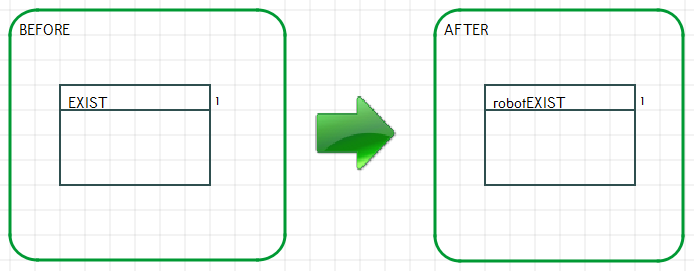
\includegraphics[width=0.6\textwidth]{part4/refactoringExample.png}
		\caption{Пример правила рефакторинга, дописывающего префикс "`robot"' к имени узла.}
		\label{image:refactoringExample}
	\end{center}
\end{figure}

После того, как правило создано, оно сохраняется (в виде обычного файла сохранения QReal), 
и при создании диаграммы на языке, для которого оно было определено, может быть применено. 
Для этого пользователю доступно диалоговое окно, в котором он может выбрать применяемый 
рефакторинг, найти следующее соответствие шаблона рефакторинга в диаграмме и применить 
рефакторинг к найденному соответствию. Внешний вид этого диалогового окна представлен 
на рисунке~\ref{image:refactoringSelectionWindow}.

\begin{figure} [ht]
	\begin{center}
		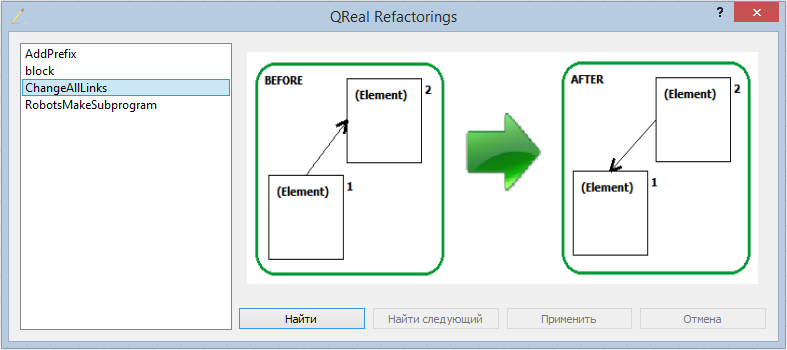
\includegraphics[width=0.9\textwidth]{part4/refactoringSelectionWindow.png}
		\caption{Диалоговое окно применения рефакторинга, с рефакторингом "`обращение всех связей"'.}
		\label{image:refactoringSelectionWindow}
	\end{center}
\end{figure}

С технической точки зрения средство применения рефакторингов использует тот же механизм 
работы с графовыми грамматиками, что и используемый для задания семантики интерпретации 
визуальных языков. Этот механизм, а также существующие его аналоги, подробно описан в статьях
%TODO: Ссылка
% Поляков В.А., Брыксин Т.А. Подходы к заданию семантики интерпретации диаграмм, основанные на технологии преобразования графов // Компьютерные инструменты в образовании, СПб., 2013, № 2, С. 3-17
% Поляков В.А., Брыксин Т.А. Средство разработки визуальных интерпретаторов и отладчиков диаграмм в проекте QReal // Материалы межвузовского конкурса-конференции студентов, аспирантов и молодых ученых Северо-Запада "Технологии Microsoft в теории и практике программирования". СПб.: Изд-во СПбГПУ, 2013. С. 80-81
% Поляков В.А., Брыксин Т.А., Подходы к заданию семантики интерпретации диаграмм в рамках DSM-подхода // Системное программирование, Вып. 7. СПб.: Изд-во СПбГУ. 2012. С. 187-216.
% Поляков В.А., Разработка визуального интерпретатора моделей в системе QReal // Список-2012: Материалы всероссийской научной конференции по проблемам информатики. 25-27 апр. 2012г., Санкт-Петербург. — СПб.: Изд-во ВВМ, 2012. С. 56-61
 и в диссертации Брыксина Т.А.
%TODO: Ссылка.
. Физически средство применения рефакторингов реализовано как подключаемый модуль к 
QReal, поскольку, в отличие от подсистемы проверки ограничений, не требует тесной 
интеграции с ядром системы.

\section{Средства поддержки технологии "`метамоделирования на лету"'}
Технология "`метамоделирования на лету"' позволяет разрабатывать предметно-ориентированные 
языки не используя метаредактор, прямо в процессе рисования диаграммы на разрабатываемом 
языке. Методологические аспекты технологии, включая описание процесса создания языка 
в соответствии с ней, описаны в разделе~\ref{chapter:MetamodelingOnFly} настоящей 
работы, здесь будет кратко описана реализация инструментальных средств поддержки этой 
технологии в системе QReal, выполненная под руководством автора Птахиной Алиной Ивановной 
в рамках курсовой работы. Подробное описание реализации можно найти в тексте курсовой работы 
%TODO: Ссылка.
и в статье
%TODO: Ссылка.
% Птахина А.И. Разработка метамоделирования “на лету” в системе QReal // Список-2013: Материалы всероссийской научной конференции по проблемам информатики. 2013г ., Санкт-Петербург. — СПб.: Изд-во ВВМ, 2012. С. 28-36
.

Метамоделирование на лету --- это особый режим работы QReal, не доступный при работе 
с такими технологиями, как QReal:Robots. Таким образом, пользователи предметно-ориентирвоанных 
решений, созданных на основе QReal, имеют возможность даже не знать о существовании 
такой функциональности. Если же QReal запущен в режиме DSM-платформы, на стартовом 
экране будет предложено выбрать между метаредактором, или созданием или открытием 
интерпретируемой метамодели, как показано на рисунке~\ref{image:qRealStartScreen}.

\begin{figure} [ht]
	\begin{center}
		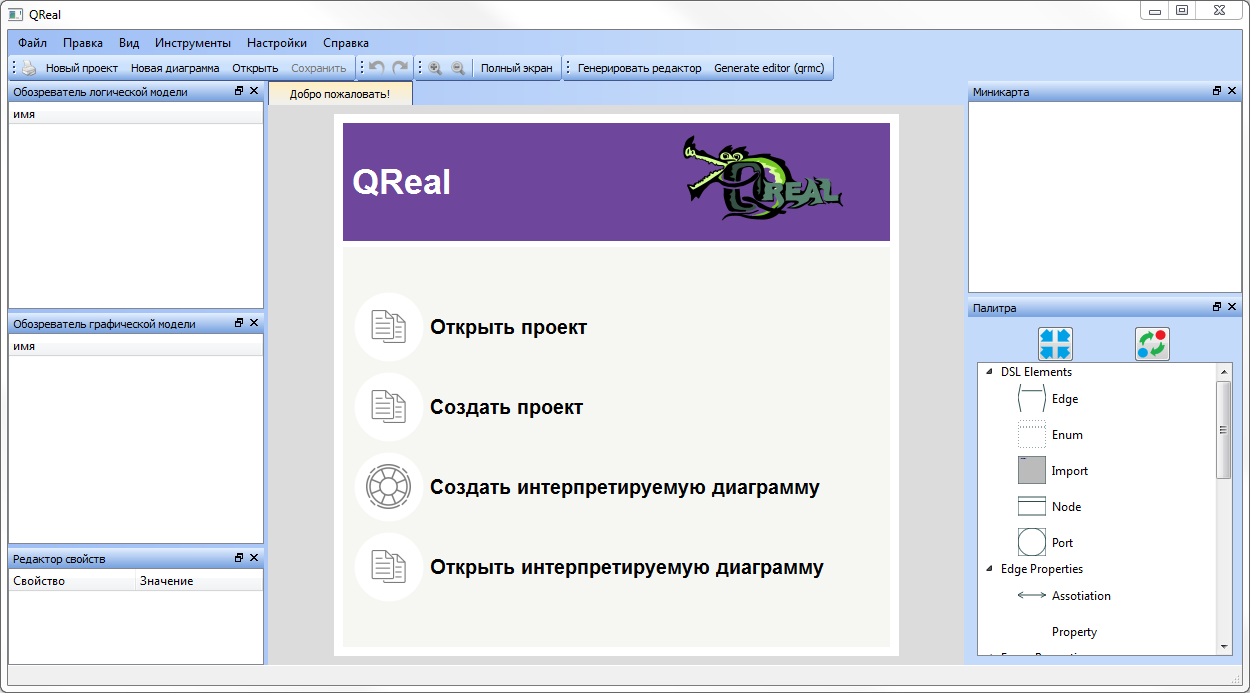
\includegraphics[width=\textwidth]{part4/qRealStartScreen.png}
		\caption{Стартовый экран QReal.}
		\label{image:qRealStartScreen}
	\end{center}
\end{figure}

При выборе пункта меню "`Открыть интерпретируемую диаграмму"' будет предложено выбрать 
файл сохранения с метамоделью языка, которая будет загружена в интерпретатор, после 
чего будет создана пустая модель с этой метамоделью. При желании можно после этого 
загрузить файл с сохранённой моделью, созданной с помощью языка, метамодель которого 
загружена. При выборе пункта меню "`Создать интерпретируемую диаграмму"' будет предложено 
ввести имя создаваемого языка, после чего будет создана пустая метамодель (в среде 
при этом будет отображаться пустая палитра элементов) и пустая модель.

Элемент можно добавить в язык, кликнув правой кнопкой мыши на палитру и выбрав в контекстном 
меню пункт "`Добавить элемент"'. После этого надо выбрать метатип создаваемого элемента 
--- сущность или связь, и ввести его имя. Если создаваемый элемент --- сущность, его
можно пометить как корневой элемент диаграммы, в этом случае он будет создаваться 
автоматически при создании диаграммы, и только он может быть в корне иерархии включения 
элементов (то есть это тот элемент, в который как в сыновья добавляются все остальные, 
это обычно и есть узел "`диаграмма"' для языка). Вновь созданный элемент будет иметь 
форму по умолчанию (прямоугольник для сущностей и обычную линию для связей) и не будет 
иметь свойств. Элемент уже можно начать использовать, например, если это корневой 
элемент нового языка, перетащить в "`Обозреватель графической модели"', что приведёт 
к созданию новой диаграммы, куда можно добавлять этот же или другие элементы. Форму 
элемента можно поменять, кликнув по элементу на палитре или на диаграмме правой кнопкой 
и выбрав пункт "`Изменить внешний вид"' в контекстном меню. Схематически данный процесс 
показан на рисунке~\ref{image:metamodelingOnFlyCreationOfElement}.

\begin{figure} [ht]
	\begin{center}
		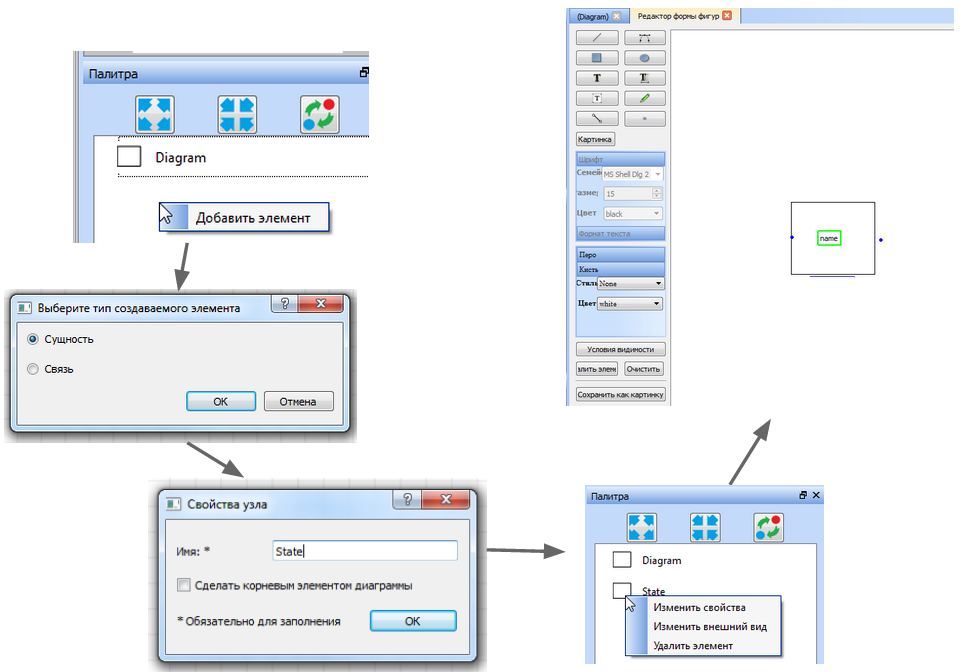
\includegraphics[width=\textwidth]{part4/metamodelingOnFlyCreationOfElement.png}
		\caption{Создание нового элемента языка.}
		\label{image:metamodelingOnFlyCreationOfElement}
	\end{center}
\end{figure}

Свойства элемента также можно добавить, удалить или отредактировать через контекстное 
меню. При этом появится диалоговое окно со списком свойств. Свойства характеризуются 
своим именем, типом и значением по умолчанию. При создании нового свойства эти характеристики 
надо будет ввести, для существующих свойств их можно редактировать. При этом есть 
некоторые ограничения, связанные с поддержанием консистентности модели. Например, 
элементам, экземпляры которых уже существуют на диаграмме, нельзя добавить новое свойство 
--- уже существующие экземпляры добавленного свойства иметь не будут, что может привести 
к ошибкам в инструментальных средствах, которые рассчитаны на то, что все обозначенные 
в метамодели свойства у экземпляров элементов есть. В таком случае система запрещает 
добавление свойства и требует, чтобы до добавления свойства все экземпляры были удалены. 
При этом удаление свойства элемента безопасно --- существующие экземпляры будут иметь 
удалённое свойство, но оно никогда не будет запрошено, поскольку отсутствует в метамодели. 
Эти проблемы напрямую связаны с проблемой совместной эволюции моделей и метамодели языка, 
поскольку они будут проявляться и при открытии файла сохранения с моделью, выполненной в 
старой версии языка. На данный момент эти проблемы решаются в рамках отдельного исследования. 
Процесс редактирования свойства элемента схематически представлен на рисунке~\ref{image:metamodelingOnFlyPropertiesEditing}

\begin{figure} [ht]
	\begin{center}
		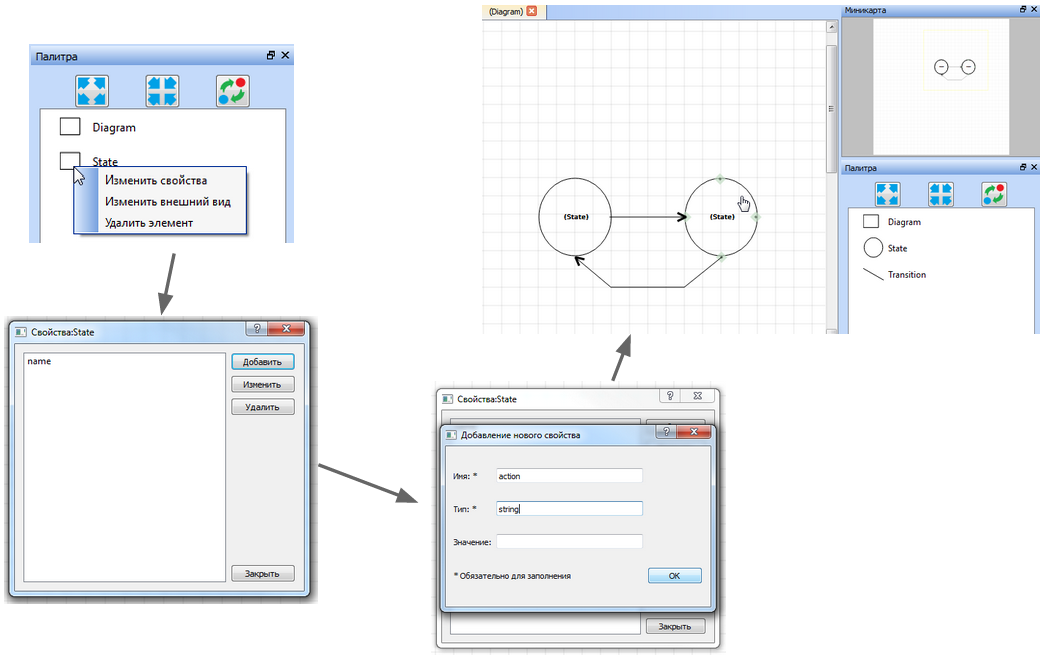
\includegraphics[width=\textwidth]{part4/metamodelingOnFlyPropertiesEditing.png}
		\caption{Редактирование свойств элемента.}
		\label{image:metamodelingOnFlyPropertiesEditing}
	\end{center}
\end{figure}
